\documentclass[a4paper,12pt]{article}
\usepackage{fancyhdr}
\usepackage{color}
\usepackage[a4paper,top=2.8cm,bottom=1cm,left=1.2 in,right=1.4 in]{geometry}
\usepackage{caption}
\usepackage{amssymb}
\usepackage{graphicx}
\usepackage{wrapfig}
\usepackage{lipsum}
\pagestyle{fancy}
\usepackage{fancyhdr}
\fancyhf{}             
\usepackage{lipsum}
\usepackage{amsmath}
\usepackage{xcolor}
\usepackage{times}
\usepackage{setspace}
\usepackage{newtxtext,newtxmath}
\fancyhf{} 
\renewcommand{\headrulewidth}{0pt}
\fancyhead[L]{
        
\includegraphics[width=6cm, height=1.7cm]{comet.jpeg} 
        }
\fancyhead[R]{
    Name: G.MADHU LATHA \\
    Batch: COMETFWC029\\
    Date: 21 MAY-2025
}

\renewcommand{\headrulewidth}{0pt}
\makeatletter
\def\headrule{%
  {\color{cyan}%
   \hrule width\headwidth height 1pt  \vskip-1pt} 
}
\setlength{\headheight}{3cm}
\begin{document}
\makeatother
\begin{spacing}{2.5}
\noindent Now,
\hspace{5em}$
\tan 45^\circ = \frac{AE}{DE}$ \\
i.e,
\hspace{7em} $ 1=\frac{AE}{28.5}$ \\
Therefore,
\vspace{-4em}
\hspace{3em} $ AE = 28.5 $ \\
\end{spacing}
\noindent So the height of the chimney(AB)=$(28.5+1.5)m $ \\
\vspace{-0.9em}

\noindent
\textcolor{cyan}{\textbf{Example 4:}}
From a point $P$ on the ground, the angle of elevation of the top of a $10\,\text{m}$ tall building is $30^\circ$. A flag is hoisted at the top of the building and the angle of elevation of the top of the flagstaff from $P$ is $45^\circ$. Find the length of the flagstaff and the distance of the building from the point $P$. (You may take $\sqrt{3} = 1.732$) \\
\vspace{0.15em}

\noindent\textcolor{cyan}{\textbf{Solution:}}In Fig. 9.7, $AB$ denotes the height of the building, $BD$ the flagstaff, and $P$ the given point. Note that there are two right triangles $PAB$ and $PAD$. We are required
to find the length of the flagstaff, i.e., $DB$ and the distance of the building from the
point $P$, i.e.,$PA$.
\hfill
\begin{minipage}[t]{0.5\textwidth}
\vspace{1em}
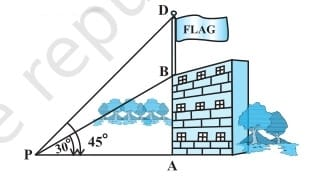
\includegraphics[height=5cm, width=\linewidth]{task21.jpeg}
\begin{center}
\vspace{-0.5em}
\textcolor{cyan}{\textbf{Fig. 9.8}}
\end{center}
\end{minipage}


\vspace{-12em}
Since we know the height of the building AB,\\
we will first consider the right $  \triangle PAB. $ 
\begin{spacing}{2.5}
\noindent
We have 
\hspace{2em} 
$ \tan 30^\circ = \frac{AB}{AP}$ \\
i.e, \hspace{4em}
$ \frac{1}{\sqrt{3}} = \frac{10}{AP} $\\
Therefore,
\hspace{1em}
$ AP=10 \sqrt{3}$ \\
i.e.,the distance of the building from P is $ 10\sqrt{3}m $ =$17.32m $. \\
Next, let us suppose $DB = x m$. Then AD = $(10 + x) m.$ \\
Now,in right $\triangle PAD$ ,
\hspace{1em}
$\tan 45^\circ $ =$ \frac{AD}{AP}$=$\frac{10+x}{10\sqrt{3}}$ \\
Therefore,\hspace{6em} 1=$\frac{10+x}{10\sqrt{3}}$ \\
\end{spacing}
\begin{center}
\vspace{1em}
2019-20
\end{center}
\newpage
\lhead{\textcolor{cyan}{\textbf{SOME APPLICATIONS OF TRIGONOMETRY}}}
\rhead{\textcolor{cyan}{\textbf{201}}}
\noindent i.e,\vspace{0.8em}
\hspace{4em} $x=10(\sqrt{3}-1)=7.32 $\\
\vspace{1em}
So,the length of the flagstaff is 7.32m.

 \noindent\begin{minipage}[t]{0.5\textwidth}
 \textbf{\textcolor{cyan}{Example 5 :}} The shadow of a tower standing on a level ground is found to be 40 m longer when the Sun’s altitude is $30^\circ$ than when it is $60^\circ$. Find the height of the tower.

\vspace{1em}

\textbf{\textcolor{cyan}{Solution :}} In Fig. 9.8, AB is the tower and BC is the length of the shadow when the Sun’s altitude is $60^\circ$, i.e., the angle of elevation of the top of the tower from the tip of the shadow is $60^\circ$ and DB is the length of the shadow, when the angle of elevation is $30^\circ$.
\end{minipage}
\hfill
\begin{minipage}[t]{0.38\textwidth}
\vspace{-1em}
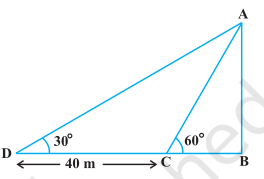
\includegraphics[height=5cm,width=\linewidth]{task22.png}

\begin{center}
\vspace{-1em}
\textcolor{cyan}{\textbf{Fig. 9.8}}
\end{center}
\end{minipage}
\noindent 
\vspace{2em}
Now, let AB be h m and BC be x m. According to the question, DB is 40 m longer
than BC.\\
\begin{spacing}{2.1}
\noindent
So, \hspace{10em} $DB=(40+x)m $\\
Now,we have two right triangles ABC and ABD.\\
In $\triangle ABC$, \hspace{8em}
$\tan 60 ^\circ =\frac{AB}{BC}$\\
or,\hspace{12em}
$\sqrt{3}=\frac{h}{x}$ \hspace{15em} $(1)$\\
In $\triangle ABD$, \hspace{8em}
$\tan 30^ \circ =\frac{AB}{BC}$ \\
i.e, \hspace{11em}
$\frac{1}{\sqrt{3}}=\frac{h}{x+40}$  \hspace{14.5em} $(2)$\\
From (1),We have \hspace{5em} $h=x\sqrt{3} $ \\
Putting this value in $(2)$, we get $(x\sqrt{3})\sqrt{3}=x+40,i.e.,3x=x+40 $\\
i.e, \hspace{12em} $x=20$ \\
So, \hspace{12em} $h=20\sqrt{3}$  \hspace{13em} [From(1)]\\
Therefore, the height of the tower is$ 20\sqrt{3} m$.
\end{spacing}
\begin{center}
\vspace{1em}
2019-20
\end{center}

\end{document}